\section{Справочные сведения}\label{sec:general_information}
	\subsection{Общие сведения о походе}\label{subsec:general_information}
		\begin{longtable}{|>{\centering\arraybackslash} m{6.1cm}|>{\centering\arraybackslash} m{10cm}|} \hline
			Район похода														&	Российская Федерация, Кавказ (Безенги,~Приэльбрусье)						\\ \hline
			Вид туризма															&	Горный																		\\ \hline
			Категория сложности похода											&	Третья																		\\ \hline
			Проводящая организация												&	Горный турклуб МГУ, г.~Москва												\\ \hline
			Руководитель														&	Чашникова Анастасия Алекссандровна 											\\ \hline
			Контакты руководителя												&	тел.~+7(950)~816-39-44 e-mail:~chashni98@gmail.com 							\\ \hline
			Сроки активной части похода полные \newline (от Москвы до Москвы)	&	с 30 июня по 18 июля 2024 года \textit{(с~28~июня~по~20~июля~2024~года)}	\\ \hline
			Протяженность маршрута (по gps)									&	158.1\,км (163.6\,км с учётом радиальных выходов для части группы)			\\ \hline
			Длина маршрута с учётом $k = 1.1$ в зачёт									&	159.4\,км										\\ \hline
			Продолжительность активной части									&	19 дней																		\\ \hline
			Суммарный набор/сброс, м											&	+12550/-13070																\\ \hline
			Максимальная высота													&	4420\,м (вер. Тютю 2-ая Зап.)												\\ \hline
			Максимальная высота ночёвки											&	4185\,м (пер.~Тютю Зап.)													\\ \hline
		\end{longtable}\fxnote{Поправить километраж}
	
	
	\subsection{Запланированная нитка маршрута}\label{subsec:planned_route}
\renewcommand{\bfdefault}{bx}
		\textit{%
			Т/б~Уштулу~"---
			\hyperref[subsec:Day2]{пер.~Штулу + п.~Штулу (1А, рад.)}~"---
			д.р.~Карасу~"---
			приют Уштулу~"---
			д.р.~Черек Балкарский~"---
			д.р.~Тютюнсу~"---
			\hyperref[subsec:Day4]{пер.~Туристов Грузии + пер. Ашинова (1Б)}~"---
			лед.~Крумкол~"---
			\hyperref[subsec:Day6]{пер.~Спартак + п.~Башхауз + пер.~МВТУ (2А)} "---
			а/л~Безенги~"---
			\hyperref[subsec:Day11]{пер.~Столбовой (2А)}~"---
			\hyperref[subsec:Day12]{пер.~Тютюргу (1Б)}~"---
			\hyperref[subsec:Day12]{пер.~Шаурту + п. МВТУ (2А)}~"---
			лед.~Шаурту~"---
			д.р.~Тютюргу~"---
			д.р.~Гара-Аузу-Су~"---
			д.р.~Башиль-Аузу-Су~"---
			т/б Башиль~"---
			д/р~Джайлык-Су~"---
			лед.~Джайлык~"---
			\hyperref[subsec:Day16]{пер.~Кенчат + п.~Кенчатбаши + пер.~Килар (2А)}~"---
			лед.~Кенчат Западный~"---
			ночевки Тютю нижние~"---
			\hyperref[subsec:Day17]{пер.~Тютю Зап. + п.~Тютюбаши 2-ая Зап. + пер.~Куллумкол + пер. Шогенцукова (2А)}~"---
			д/р~Куллумкол-Су~"---
			а/л~Джайлык~"---
			Верхний Баксан.%
		}
		\fxnote{Поправить ссылки!}
		\fxnote{Поправить тире! не видны на нормальном масштабе!}
	
	\subsection{Пройденная нитка маршрута}\label{subsec:real_route}
		\textit{%
			Т/б~Уштулу~"---
			\hyperref[subsec:Day2]{пер.~Штулу + п.~Штулу (1А, рад.)}~"---
			д.р.~Карасу~"---
			приют Уштулу~"---
			д.р.~Черек Балкарский~"---
			д.р.~Тютюнсу~"---
			\hyperref[subsec:Day4]{пер.~Туристов Грузии + пер. Ашинова (1Б)}~"---
			лед.~Крумкол~"---
			\hyperref[subsec:Day6]{пер.~Спартак + п.~Башхауз + пер.~МВТУ (2А)}~"---
			а/л~Безенги~"---
			\hyperref[subsec:Day11]{пер.~Столбовой (2А)}~"---
			\hyperref[subsec:Day12]{пер.~Тютюргу (1Б)}~"---
			\hyperref[subsec:Day12]{пер.~Шаурту (2А)}~"---
			лед.~Шаурту~"---
			д.р.~Тютюргу~"---
			д.р.~Гара-Аузу-Су~"---
			д.р.~Башиль-Аузу-Су~"---
			т/б Башиль~"---
			д/р~Джайлык-Су~"---
			\hyperref[subsec:Day16]{пер.~Надежда (1Б, п/п) + пер. Кенчат + п.~Кенчатбаши (2А, рад.)}~"---
			\hyperref[subsec:Day16]{пер.~Килар (1Б)}~"---
			лед.~Кенчат Западный~"---
			ночевки Тютю нижние~"---
			\hyperref[subsec:Day17]{пер.~Тютю Зап. + п.~Тютюбаши 2-ая Зап. + пер.~Куллумкол + пер.~Шогенцукова (2А)}~"---
			д/р~Куллумкол-Су~"---
			а/л~Джайлык~"---
			Верхний Баксан.%
		}
		\fxnote{Поправить ссылки!}
		\renewcommand{\bfdefault}{b}
		
		Маршрут пройден с изменениями, подробнее см. \ref{subsec:changes_of_way}.

	
	\subsection{Характеристика препятствий}\label{subsec:main_obstacles}

		\setlength{\arraycolsep}{0.5pt}
		\renewcommand{\arraystretch}{1}
		{\small\begin{longtable}{|>{\centering\arraybackslash}m{3.8cm}|>{\centering\arraybackslash}m{1.3cm}|>{\raggedright\arraybackslash}m{11.5cm}|>{\centering\arraybackslash}m{1cm}|} \hline
		 	Препятствие																																	&	Кат. трудн., высота			&	Краткое описание																																																																																																																																																																																										&	ЧХВ		\\ \hline
		 	\hyperref[subsec:Day2]{Пер.~Штулу~+ п.~Штулу}														\newline\textit{радиально с запада}		&	1А, 3570					&	Подъем на перевал Штулу "--- зямлянисто-травяной склон до $25^\circ$, короткие участки снежников до $15^\circ$. Путь от перевала до вершины проходит по сланцевой осыпи крутизной до $25^\circ$, также встречаются короткие участки пологих снежников. \newline \textbf{Вывод:} Связка пер. Штулу + вер. Штулу-Тау соответствуют категории 1А и могут быть рекомендованы группам, совершающим походы 1 к.с. и выше. Препятствие отлично подходит для акклиматизации группы. 																																																																																																																																																						&			\\ \hline
		 	\hyperref[subsec:Day4]{Пер.~Туристов Грузии~+ пер.~Ашинова}											\newline\textit{с севера на юг}			&	1Б, 3640 3720				&	Подход по долине реки Тютюнсу под перевал Туристов Грузии трудоемок, большая его часть проходит по заросшей тропе. Встречаются участки заросших кустарниками каменистых склонов на прижимах реки, участки высокой тропы, заросли низкорослых деревьев. Подъем на перевал Туристов Грузии проходит по снежному склону до $25^\circ$ и не требует движения в кошках или подстраховку ледорубом. Есть очень короткие участки, на которых в менее снежное время года и в более ясную погоду есть вероятность схода камней. Седловина перевала широкая, снежно-осыпная, здесь вполне можно разбить лагерь. Спуск осуществляем в связках по леднику до $20^\circ$, преимущественно ледник закрытый. Подъем на перевал Ашинова проходит по снежному склону крутизной до $30^\circ$, движемся с самостраховкой ледорубом. Выкаты довольно пологие и безопасные. Седловина перевала очень широкая, мелкоосыпная, с нее открываются прекрасные виды на ГКХ, в котором доминируют отдельно стоящая Айлама и Шхара, с которой начинается Безенгийская стена. С другой стороны отлично виден массив Суганского хребта. Спуск проходит по мелколифтовой осыпи, несколько раз пересекаем участки подмерзших с ночи снежников до $25^\circ$, движемся в кошках с самостраховкой ледорубом. \newline	\textbf{Вывод:} Связка пер. Туристов Грузии + пер. Ашинова соответствуют 1Б категории сложности. Эти препятствия целесообразно включать в походы от 3 к.с. Перевалы также подходят для акклиматизации и позволяют вспомнить навыки движения по некрутому снегу, в кошках, движение в связках.																																																																																																																					&			\\ \hline
			\hyperref[subsec:Day6]{Пер.~Спартак~+ п.~Башхауз~ + пер.~МВТУ}										\newline\textit{с севера на юг}			&	2А, 4090 4410 4215			&	Подъем на перевал осуществляем по леднику Крумкол, сам ледник пологий, до $15^\circ$. Необходимо пересечь зону разломов, здесь встречаются короткие участки льда до $45^\circ$, которы преодолеваем с попеременной страховкой через ледобуры или с одновременной страховкой в связках. Стоит отметить, что прохождение ледопада возможно только при хорошей видимости. Довольно много широких трещин ранним июльским утром мы перешли по плотным и надежным снежным мостам. Перевальный взлет короткий, до $25^\circ$, проходим в связках. Подъем на гребень вершины Башхауз требует уверенных навыков гребневого лазанья, встречаются достаточно узкие участки гребня, участки простых разрушенных скал. Организуем перильную страховку на траверсе снежников. На слияние Ю и ЮВ гребня поднимаемся по кулуару разррушенных скал крутизной до $45^\circ$, организуем перильную страховку на скальных выступах. Для перехода с Ю на ЮВ организуем короткий участок перильной страховки (до 10 м). Спуск по Ю гребню к перевалу МВТУ проходит по протоптанной альпинистской тропе на осыпи крутизной до $30^\circ$. Спуск с перевала МВТУ осуществляется по заснеженному кулуару до $30^\circ$, пересекаем 2 забитые трещины. Вешаем 1 веревку до выполаживания, еще 1 для подстраховки от проваливания в трещины. Станции организуем на скальном выступе, на ледорубах и на ледобурах. \newline \textbf{Вывод:} Связка пер. Спартак + вер. Башхауз + пер. МВТУ соответствует сильной 2А и очень разнообразна по рельефу: простой ледопад на подъем, скальный гребень вершины Башхауз, снежный кулуар на спуск с пер. МВТУ. Препятствие интересно технически, достаточно красивое. Мы не рекомендуем включать этот перевал как первое препятствие в походах 3 к.с. Рекомендуем проходить данное препятствие только при хорошей видимости. В августе, сложность препятствия может увеличиться, если снежные мосты растают и ледопад станет более разорванный.																											&			\\ \hline
		 	\hyperref[subsec:Day11]{Пер.~Столбовой}																\newline\textit{с востока на запад}		&	2А, 3690					&	Подход к перевалу проходит по крутому травянистому склону  до $35^\circ$, затем по полями слежавшегося курумника. Подъем на перевал с ЮВ по подвижной средней осыпи крутизной до $35^\circ$. Траверс с пер. Столбовой через вершину 50-летия КБАССР до более восточной седловины проходит по крупной осыпи, жандармы обходим слева ПХД. Спуск по леднику крутизной до $35^\circ$, преимущественно открытому, осуществляем в кошках, с перильной страховкой. Первая веревка короткая, для подстраховки при выходе с осыпи на ледник. Затем вешаем еще 4 для спуска по леднику. \newline \textbf{Вывод:} Перевал Столбовой соответствует категории трудности 2А и может быть рекомендован группам совершающим поход 3 к.с. В июле при прохождении СЗ склона по леднику камнеопасность отсутствует. Мы не рекомендуем прохождение СЗ склона по осыпи в обход ледника, так как со склонов вершины Сарыкая регулярно происходят сходы камней.																																																																																																																																																																																																																																																																															&			\\ \hline
			\hyperref[subsec:Day12]{Пер.~Тютюргу}																\newline\textit{с севера на юг}			&	1Б, 3835					&	Выход на ледник Булунгу, проходит по зачехленному языку ледника, крутизной до $25^\circ$, есть выходы льда, движемся аккуратно, в ботинках. Ледник Булунгу пологий и открытый. Подъем на перевал по короткому участку снежника до $30^\circ$, движемся с самостраховкой ледорубом. Вначале спуск по крупной осыпи, затем осыпь меняется на среднюю и мелкую, крутизна до $35^\circ$. Спуск осуществляем плотной группой \newline \textbf{Вывод:} Перевал Тютюргу соответствует категории 1Б и может быть рекомендован группам 2 к.с. Перевал требует уверенных навыков передвижения по разным видам осыпей.																																																																																																																																																																																																																																																																																																																																																															&			\\ \hline
			\hyperref[subsec:Day12]{Пер.~Шаурту}																\newline\textit{с севера на юг}			&	2А,	4085					&	Ледник Тютюргу закрытый, движемся в связках, преодолеваем 2 зоны трещин. С ледника поднимаемся на С скальный гребень, из-за мокрого снега не лезем на гребень напрямую, а обходим по осыпным кулуарам. При подъеме провешиваем 3 веревки - 2 траверс через осыпь и выходы скальных плит, 1 по осыпному кулуару на гребень. Станции организуем на скальных выступах. Осыпь очень подвижная, встречаются участки простого лазанья на протяжении всего подъема. Крутизна склона до $35^\circ$. Траверс по С гребню до перевала проходит по разрушенному скально-осыпному гребню. Спуск по средней осыпи до $30^\circ$ плотной группой. \newline \textbf{Вывод:} Перевал Шаурту при выбранной нами траектории подъема соответствует несложному перевалу 2А, может быть рекомендован группам, совершающим поход 3 к.с. Перевал рекомендуем проходить в ясную погоду, так как движение по мокрым скалам может увеличить сложность препятствия.																																																																																																																																																																																																																																																																															&			\\ \hline
			\hyperref[subsec:Day16]{Пер.~Надежда + Пер.~Кенчат~+ п.~Кенчатбаши}									\newline\textit{с севера на юг}			&	2А, 3904 3905 4090			&	Подъем на перевал Надежда по смерзшемуся снежнику вначале более пологому, ближе к перевалу крутизна доходит до $40^\circ$, преодолеваем в кошках с самостраховкой ледорубом. Седловина перевала осыпная, узкая. Спуск проходит по средней и мелкой подвижной осыпи крутизной до $30^\circ$, встречаются выходы конгломерата. Подъем на северную седловину перевала Кенчат в начале по осыпному склону $25^\circ$, затем по смерзшимся снежникам до $35^\circ$, проходим индивидуально с самостраховкой ледорубом. Седловина перевала широкая, осыпная, с запада прилегает ледник Кенчат Западный, есть небольшое озеро в мульде. На траверсе к вершине Кенчатбаши движемся в кошках и связках, первый жандарм проходим в лоб, перелезая через разрушенные скалы и среднюю осыпь, второй жандарм обходим справа пхд, организуя ледобурную дорожку. Перед самой вершиной есть небольшие участки гребневого лазания. С Кенчатбаши открываются прекрасные виды на массив Дыхтау и Коштантау, вершины Джайлык и Тютюбаши, Эльбрус, ГКХ. Скальная часть гребня вблизи перевала Килар сильно разрушена и требует уверенных навыков гребневого лазания. Спуск проходит по крупной и средней осыпи крутизной до $35^\circ$. \newline \textbf{Вывод:} Перевал Надежда соответствует категории сложности 1Б, однако включать его в нитку маршрута как самостоятельное препятствие не целесообразно. Рекомендуем прохождение этого препятствия в связке с пер. Кенчат. Связка пер.Кенчат + вер. Кенчатбаши + пер. Килар соответствует простому препятствию 2А категории сложности и может быть рекомендована в походах 3 к.с. Траверс гребня вер. Кенчатбаши очень красивый, интересный с точки зрения улучшения личной техники гребневого лазания, движения в кошках по некрутым склонам (до $35^\circ$). В августе пер. Надежда и Ю-ЮВ склоны пер. Кенчат могут стать камнеопасными. Возможно, было бы интересно пройти траверс наоборот: осуществлять движение по СЗ склону пер. Кенчат и В склону пер. Килар. Такой траверс сложнее технически, но, возможно, безопаснее.	&			\\ \hline
			\hyperref[subsec:Day16]{Пер.~Килар}																	\newline\textit{с востока на запад}		&	1Б, 3885					&	Подъем на перевал через осыпные поля и траверс снежника крутизной до $25^\circ$. Спуск траверсом крупной осыпи с выходами разрушенных скал, встречаются элементы лазания. Крутизна до $35^\circ$. Ледник Кенчат Западный преимущественно закрытый, проходим в связках. Есть небольшая зона трещин. \newline \textbf{Вывод:} Перевал Килар соответствует категории сложности 1Б. Прохождение З склона перевала Килар достаточно неприятное и требует аккуратного движения плотной группой, чтобы избежать скидывания камней друг на друга. Мы посчитали небезопасным дюльфер по данному склону. Рекомендуем с осторожностью включать данный перевал в походы 2 к.с.																																																																																																																																																																																																																																																																																																																																																	&			\\ \hline
			\hyperref[subsec:Day17]{Пер.~Тютю~Зап.~+ п.\,Тютюбаши\,2\,Зап.\,+ пер.~Куллумкол~+ пер.~Шогенцукова}	\newline\textit{с севера на юг}			&	2А,	4185 4300 3915 3590		&	Подъем по леднику Тютю осуществляем в связках. Так как середина июля - многие трещины забиты снегом. Трещины несложно перейти по мостам, крутые ледовые участки на траверсе (до $30^\circ$) проходим с ледобурной дорожкой. Наиболее крутой участок (до $40^\circ$) проходим с перильной страховкой. Перед выходом в перевальный цирк переходим крупный бергшрунд по надежному снежному мосту. Перевальный взлет короткий, снежный, крутизной до $25^\circ$. На гребне можно поставить палатки, это отличная обзорная точка. Лучшие утренние панорамы сделаны именно отсюда. На вершину Тютюбаши 2-ая Западная поднимаемся по снежно-осыпному гребню, крутизна до $35^\circ$. Траверс к пер. Куллумкол проходит по натоптанной альпинистской тропе, но так как проходили препятствие в начале сезона, в некоторых местах нужно быть аккуратными с выходами обледенелых снежников. Встречаются участки простого лазания. Спуск с перевала Куллумкол к пер. Шогенцукова и далее в долину реки Куллумкол-Су проходит по альпинистской тропе, и несмотря на то, что частично проходит по ледникам, не требует кошек или ледоруба. \newline \textbf{Вывод:} Связка пер. Тютю зап.+ вер. Тютюбаши 2-ая Зап. + пер. Куллумкол + пер. Шогенцукова соответствует препятствию 2А категории сложности. Крайне рекомендкем включать это препятствие в походы 3 к.с., оно красивое, безопасное и технически интересное.																																																																																																																																																															&			\\ \hline
		\end{longtable}}
		\setlength{\arraycolsep}{5pt}
		\renewcommand{\arraystretch}{1.8}
		\fxnote{Доделать таблицу}
		\fxwarning{СДЕЛАТЬ ТАБЛИЦЕ ХОРОШО В ШИРИНУ!}
		

	\subsection{Состав группы}\label{subsec:group_composition}
		\begin{longtable}{|>{\centering\arraybackslash} m{3.5cm}|>{\centering\arraybackslash} m{3.6cm}|>{\centering\arraybackslash} m{3.5cm}|>{\centering\arraybackslash} m{2.5cm}|>{\centering\arraybackslash} m{2.5cm}|}\hline
			Фотография																																	&	ФИО										&	Должность					&	Год рождения	&	Опыт		\\ \hline
			\raisebox{-0.05\height}{\rule{0pt}{155pt}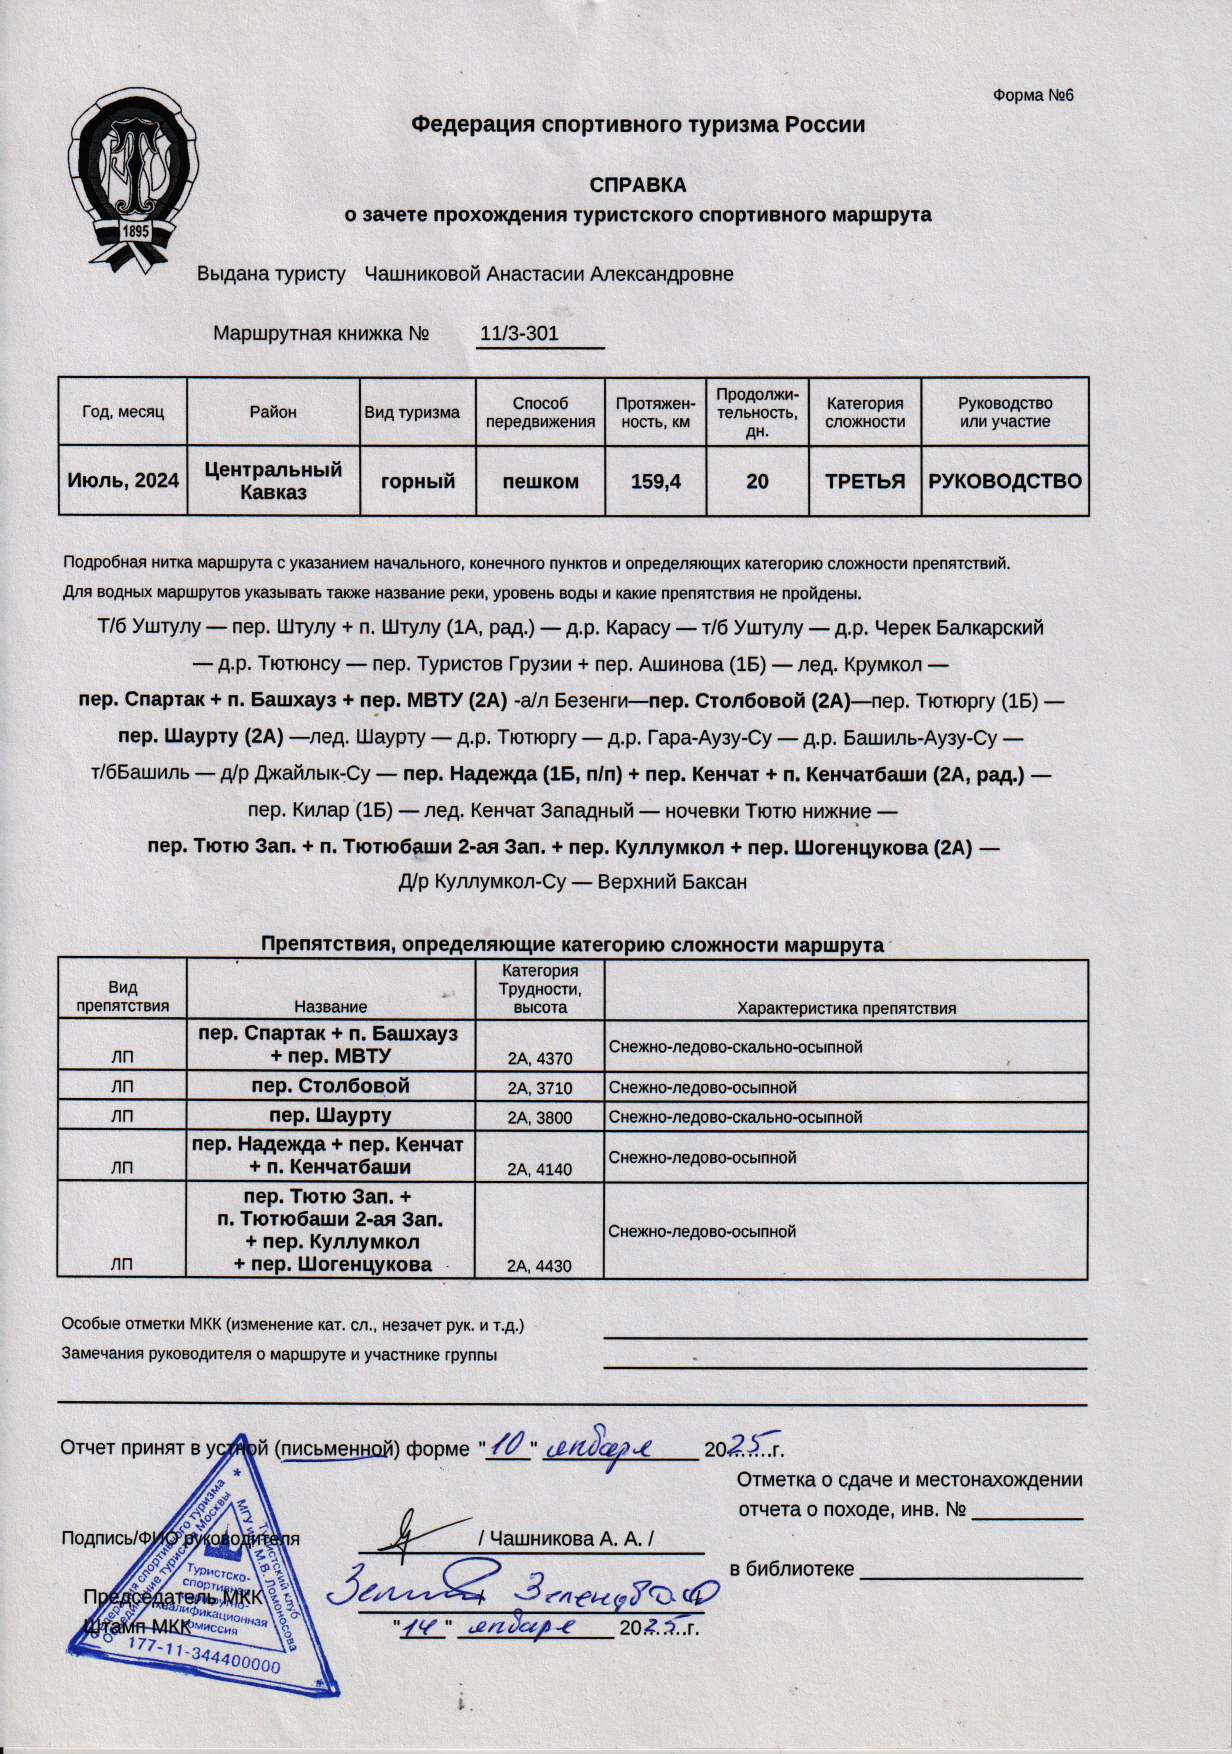
\includegraphics[width=3.5cm]{Pictures/Chapter1/Nastya.jpeg}\raisebox{-1\height}{\rule{0pt}{5pt}}}	&	Чашникова Анастасия Алекссандровна		&	Руководитель				&	1998			&	4ГУ, 2ГР	\\ \hline
			\raisebox{-0.05\height}{\rule{0pt}{155pt}\includegraphics[width=3.5cm]{Pictures/Chapter1/Dima.jpeg  }\raisebox{-1\height}{\rule{0pt}{5pt}}}	&	Коротков Дмитрий Юрьевич				&	Реммастер					&	2001			&	3ГУ, 1ГР	\\ \hline
			\raisebox{-0.05\height}{\rule{0pt}{155pt}\includegraphics[width=3.5cm]{Pictures/Chapter1/Dasha.jpeg }\raisebox{-1\height}{\rule{0pt}{5pt}}}	&	Короткова Дарья Алексеевна				&	Завпит						&	2002			&	2ГУ			\\ \hline
			\raisebox{-0.05\height}{\rule{0pt}{155pt}\includegraphics[width=3.5cm]{Pictures/Chapter1/Kate.jpeg  }\raisebox{-1\height}{\rule{0pt}{5pt}}}	&	Мерчи-Байрамова Екатерина Вячеславовна	&	Логист						&	2002			&	2ГУ			\\ \hline
			\raisebox{-0.05\height}{\rule{0pt}{155pt}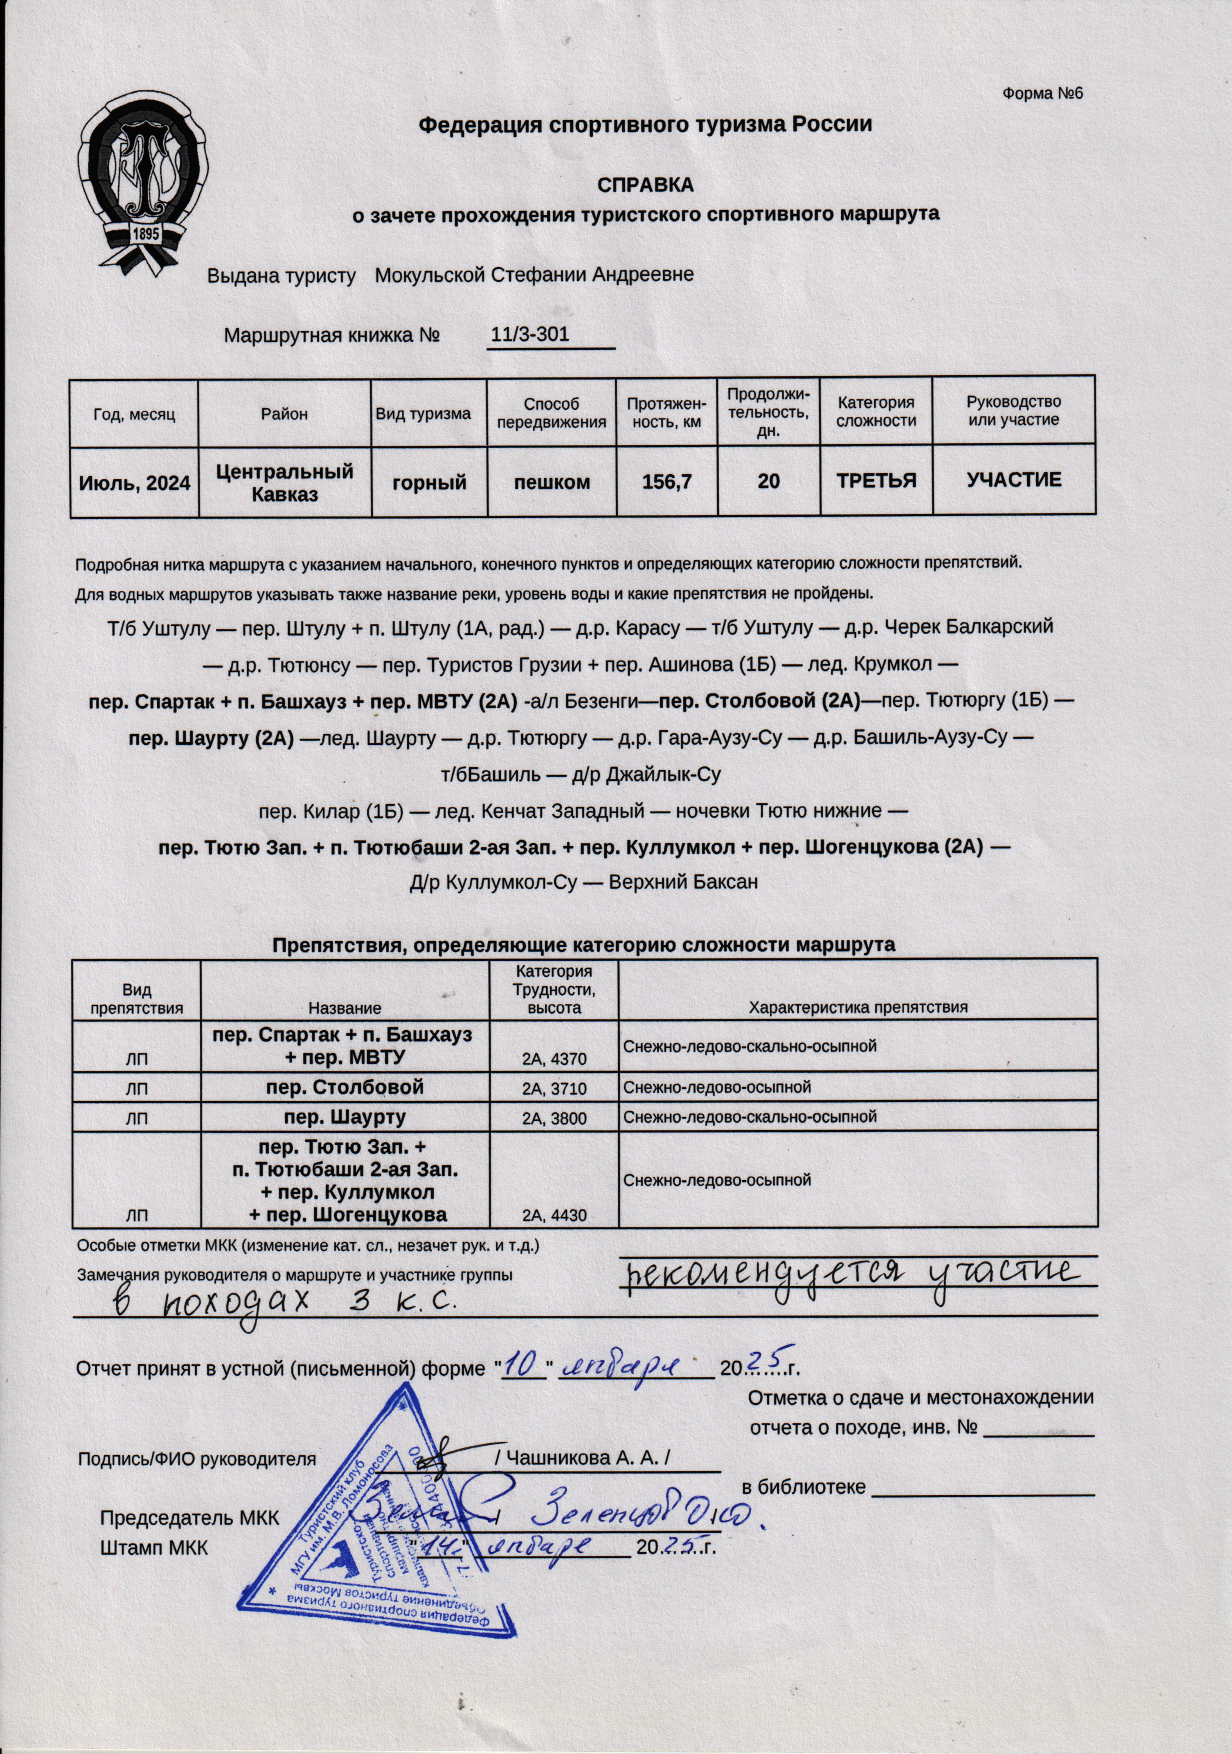
\includegraphics[width=3.5cm]{Pictures/Chapter1/Stepha.jpeg}\raisebox{-1\height}{\rule{0pt}{5pt}}}	&	Мокульская Стефания Андреевна			&	Медик, фотограф				&	1997			&	2ГУ			\\ \hline
			\raisebox{-0.05\height}{\rule{0pt}{155pt}\includegraphics[width=3.5cm]{Pictures/Chapter1/Lesha.jpeg }\raisebox{-1\height}{\rule{0pt}{5pt}}} &	Ткачёв Алексей Владимирович				&	Штурман						&	1988			&	2ГУ			\\ \hline
			\raisebox{-0.05\height}{\rule{0pt}{155pt}\includegraphics[width=3.5cm]{Pictures/Chapter1/Yura.jpeg  }\raisebox{-1\height}{\rule{0pt}{5pt}}}	&	Цимбалов Юрий Александрович				&	Снаряженец, хронометрист	&	1989			&	4ГУ			\\ \hline
		\end{longtable}
		\fxnote{Найти нормальные фотки}
		
		Поход пройден группой в полном составе. Коротков Дмитрий и Короткова Дарья не участвовали в радиальном выходе на
		вер.~Штулу-Тау (дошли до высоты 3400\,м). Коротков Дмитрий, Короткова Дарья, Мокульская Стефания не участвовали
		в радиальном выходе на пер.~Надежда + пер.~Кенчат + вер.~Кенчатбаши.
		
